\documentclass[journal,10pt,twocolumn]{article}
\usepackage{graphicx}
\usepackage[margin=0.5in]{geometry}
\usepackage[cmex10]{amsmath}
\usepackage{array}
\usepackage{booktabs}
\usepackage{mathtools}
\title{\textbf{Conic section Assignment}}
\author{P.Revathi}
\date{October 2022}


\providecommand{\norm}[1]{\left\lVert#1\right\rVert}
\providecommand{\abs}[1]{\left\vert#1\right\vert}
\let\vec\mathbf
\newcommand{\myvec}[1]{\ensuremath{\begin{pmatrix}#1\end{pmatrix}}}
\newcommand{\mydet}[1]{\ensuremath{\begin{vmatrix}#1\end{vmatrix}}}
\providecommand{\brak}[1]{\ensuremath{\left(#1\right)}}
\providecommand{\lbrak}[1]{\ensuremath{\left(#1\right.}}
\providecommand{\rbrak}[1]{\ensuremath{\left.#1\right)}}
\providecommand{\sbrak}[1]{\ensuremath{{}\left[#1\right]}}

\begin{document}

\maketitle
\paragraph{\textit{Problem Statement} - Find the area of the region bounded by the curve $x^2=y$ and the lines y=x+2 and the x axis }

\section*{\large Solution}

\begin{figure}[h]
\centering
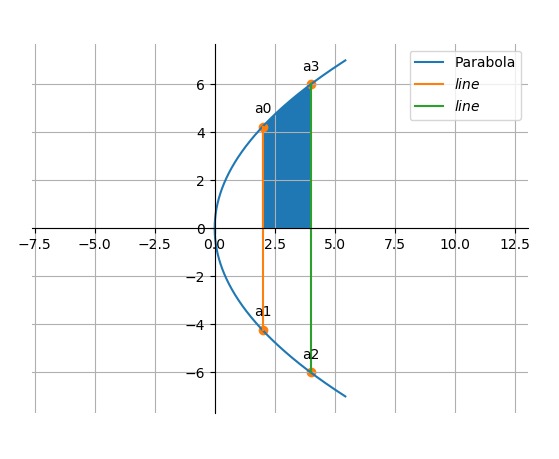
\includegraphics[width=1\columnwidth]{conics1.png}

%\caption{The parabola formed by the curve $y^2 = 9x$ and the lines x=2 and x=4}
\label{fig:parabola}
\end{figure}

The given equation of parabola $x^2 = y$ can be written in the general quadratic form as
\begin{align}
    \label{eq:conic_quad_form}
    \vec{x}^{\top}\vec{V}\vec{x}+2\vec{u}^{\top}\vec{x}+f=0
    \end{align}
where
\begin{align}
 \label{eq:V_matrix}
 \vec{V} &= \myvec{1 & 0\\0 & 0},
 \\
 \label{eq:u_vector}
 \vec{u} &= \myvec{0\\-0.5},
 \\
 \label{eq:f_value}
 f &= 0
 %\\
\end{align}

The points of intersection of the line 
\begin{align}
 L: \quad \vec{x} = \vec{q} + \mu \vec{m} \quad \mu \in \mathbf{R}
\label{eq:conic_tangent}
\end{align}
with the conic section are given by
\begin{align}
\vec{x}_i = \vec{q} + \mu_i \vec{m}
\label{eq:conic_tangent_pts}
\end{align}
%
where
{\tiny
\begin{multline}
\mu_i = \frac{1}
{
\vec{m}^T\vec{V}\vec{m}
}
\lbrak{-\vec{m}^T\brak{\vec{V}\vec{q}+\vec{u}}}
\\
\pm
\rbrak{\sqrt{
\sbrak{
\vec{m}^T\brak{\vec{V}\vec{q}+\vec{u}}
}^2
-
\brak
{
\vec{q}^T\vec{V}\vec{q} + 2\vec{u}^T\vec{q} +f
}
\brak{\vec{m}^T\vec{V}\vec{m}}
}
}
\label{eq:tangent_roots}
\end{multline}
}



From the line y=x+2 the vectors q,m are taken,
\begin{equation}
\vec{q}=\myvec{0\\2}
\end{equation}

\begin{equation}
\vec{m}=\myvec{1\\1}
\end{equation}

by substituting eq(2),(3),(4),(8),(9) in eq(7)
\begin{equation}
\mu_i=-2
\end{equation}
substituting eq(8),(9),(10) in eq(6) the intersection points on the parabola are
\begin{equation}
\vec{a_0}=\myvec{2\\4}
\end{equation}
\begin{equation}
\vec{a_1}=\myvec{-1\\1}
\end{equation}
%\begin{center}
Given line equation y=x+2\\

$$x-y=-2$$\\
$$\vec{n}^{t}\vec{x}=c$$\\
$$\vec{x}=\vec{A}+\lambda \vec{m}$$\\
%\end{centre}


$$\vec{x}=\begin{pmatrix}
-2\\ 
0
\end{pmatrix}+\mu \begin{pmatrix}
1\\ 
1
\end{pmatrix}$$\\

Substitute the x value in the quadratic equation then we get a quadratic equations
\begin{align}
    \label{eq:conic_quad_form}
    \vec{x}^{\top}\vec{V}\vec{x}+2\vec{u}^{\top}\vec{x}+f=0
    \end{align}
    
$$\mu ^{2}-3\mu +2=0\\$$
$$\mu =1,2\\$$
$$\mu ^{2}-\mu\\$$
$$\mu =1,0\\$$
The resultant x values are\\
$$\vec{x}=\begin{pmatrix}
-2\\ 
0
\end{pmatrix}$$\\
$$\vec{x}=\begin{pmatrix}
-1\\ 
1
\end{pmatrix}$$\\
$$\vec{x}=\begin{pmatrix}
0\\ 
2
\end{pmatrix}$$

Area of the parabola in between the lines parabola and y=x+2 is given by
\begin{align}
\implies A_1=\int_{-2}^{-1} \ x+2 \,dx
\end{align}

\begin{align}
\implies A_2=\int_{-1}^{0} \ x^2 \,dx
\end{align}
\begin{align}
\implies A_1+A_1=\int_{-2}^{-1} \ x+2 \,dx+\int_{-1}^{0} \ x^2 \,dx
\end{align}
\begin{align}
\implies A_1+ A_2=\frac{5}{6}sq units
\end{align}



  

\end{document}
